\documentclass[11pt,a4paper]{article}
\usepackage[margin=25mm]{geometry}
\usepackage{graphicx}
\usepackage{booktabs}
\usepackage{float}
\usepackage{hyperref}
\usepackage{caption}
\title{Physiological Stress Detection Using WESAD\\Methodology and Experimental Results}
\author{B.Tech Project}
\date{\today}

\begin{document}
\maketitle
\tableofcontents

\section{Introduction}
This report documents a reproducible physiological stress-detection system based on the WESAD dataset. The objective is to compare raw, filtered, and filtered-plus-normalized data while keeping the labels, windowing protocol, subject split, and classifier unchanged.

\section{Dataset and Signals}
The analysis uses Empatica E4 wrist signals (ACC, BVP, EDA, HR, IBI, and temperature) and RespiBAN chest signals (ACC, ECG, EDA, EMG, respiration, and temperature). Raw-signal, preprocessing, feature, and model figures are stored as PNG files in the repository's \texttt{plots/} directory.

\section{Preprocessing and Windowing}
The three variants are Raw, Filtered, and Filtered + Normalized. Signals are aligned to a common 4-Hz time base for the existing window-level ML branch. Five-second windows with 50\% overlap are labelled by the majority class. Labels 1 and 3 are treated as non-stress and label 2 as stress.

\begin{figure}[H]
\centering
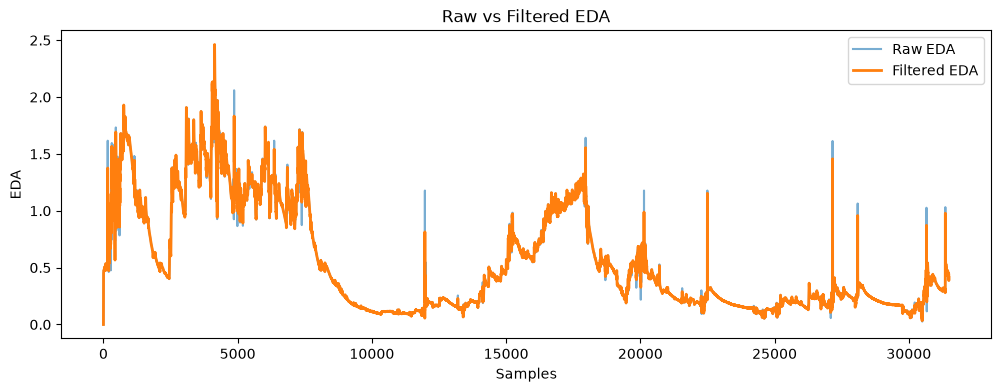
\includegraphics[width=0.95\linewidth]{figures/empatica_raw_vs_filtered_eda.png}
\caption{Example preprocessing comparison for Empatica EDA. Filtering is intended to attenuate rapid fluctuations while preserving the physiological trend.}
\label{fig:eda-filtering}
\end{figure}

\section{Feature Extraction}
Each signal channel is represented by the features actually used by the completed classical experiment: mean, median, standard deviation, variance, minimum, maximum, range, interquartile range, skewness, kurtosis, RMS, energy, entropy, mean absolute value, area under the curve, slope, zero-crossing rate, and coefficient of variation. These features describe central tendency, variability, distribution shape, magnitude, temporal trend, and signal complexity.

\begin{figure}[H]
\centering

\includegraphics[width=0.95\linewidth]{figures/feature_overview_before_model.png}
\caption{Feature overview before model fitting. This visual checks class balance and feature scale before classification.}
\label{fig:features}
\end{figure}

\section{Machine Learning Protocol}
Every signal-wise comparison uses median imputation, standardization fitted on the training data, and a class-balanced logistic-regression classifier. Evaluation is subject-independent using the fixed GroupShuffleSplit protocol with random seed 42. Accuracy, precision, recall, F1, ROC-AUC, training time, and inference time are recorded in \texttt{07\_classical\_ml/outputs/signalwise/signalwise\_model\_comparison.csv}.

\section{Experimental Results}
\begin{figure}[H]
\centering
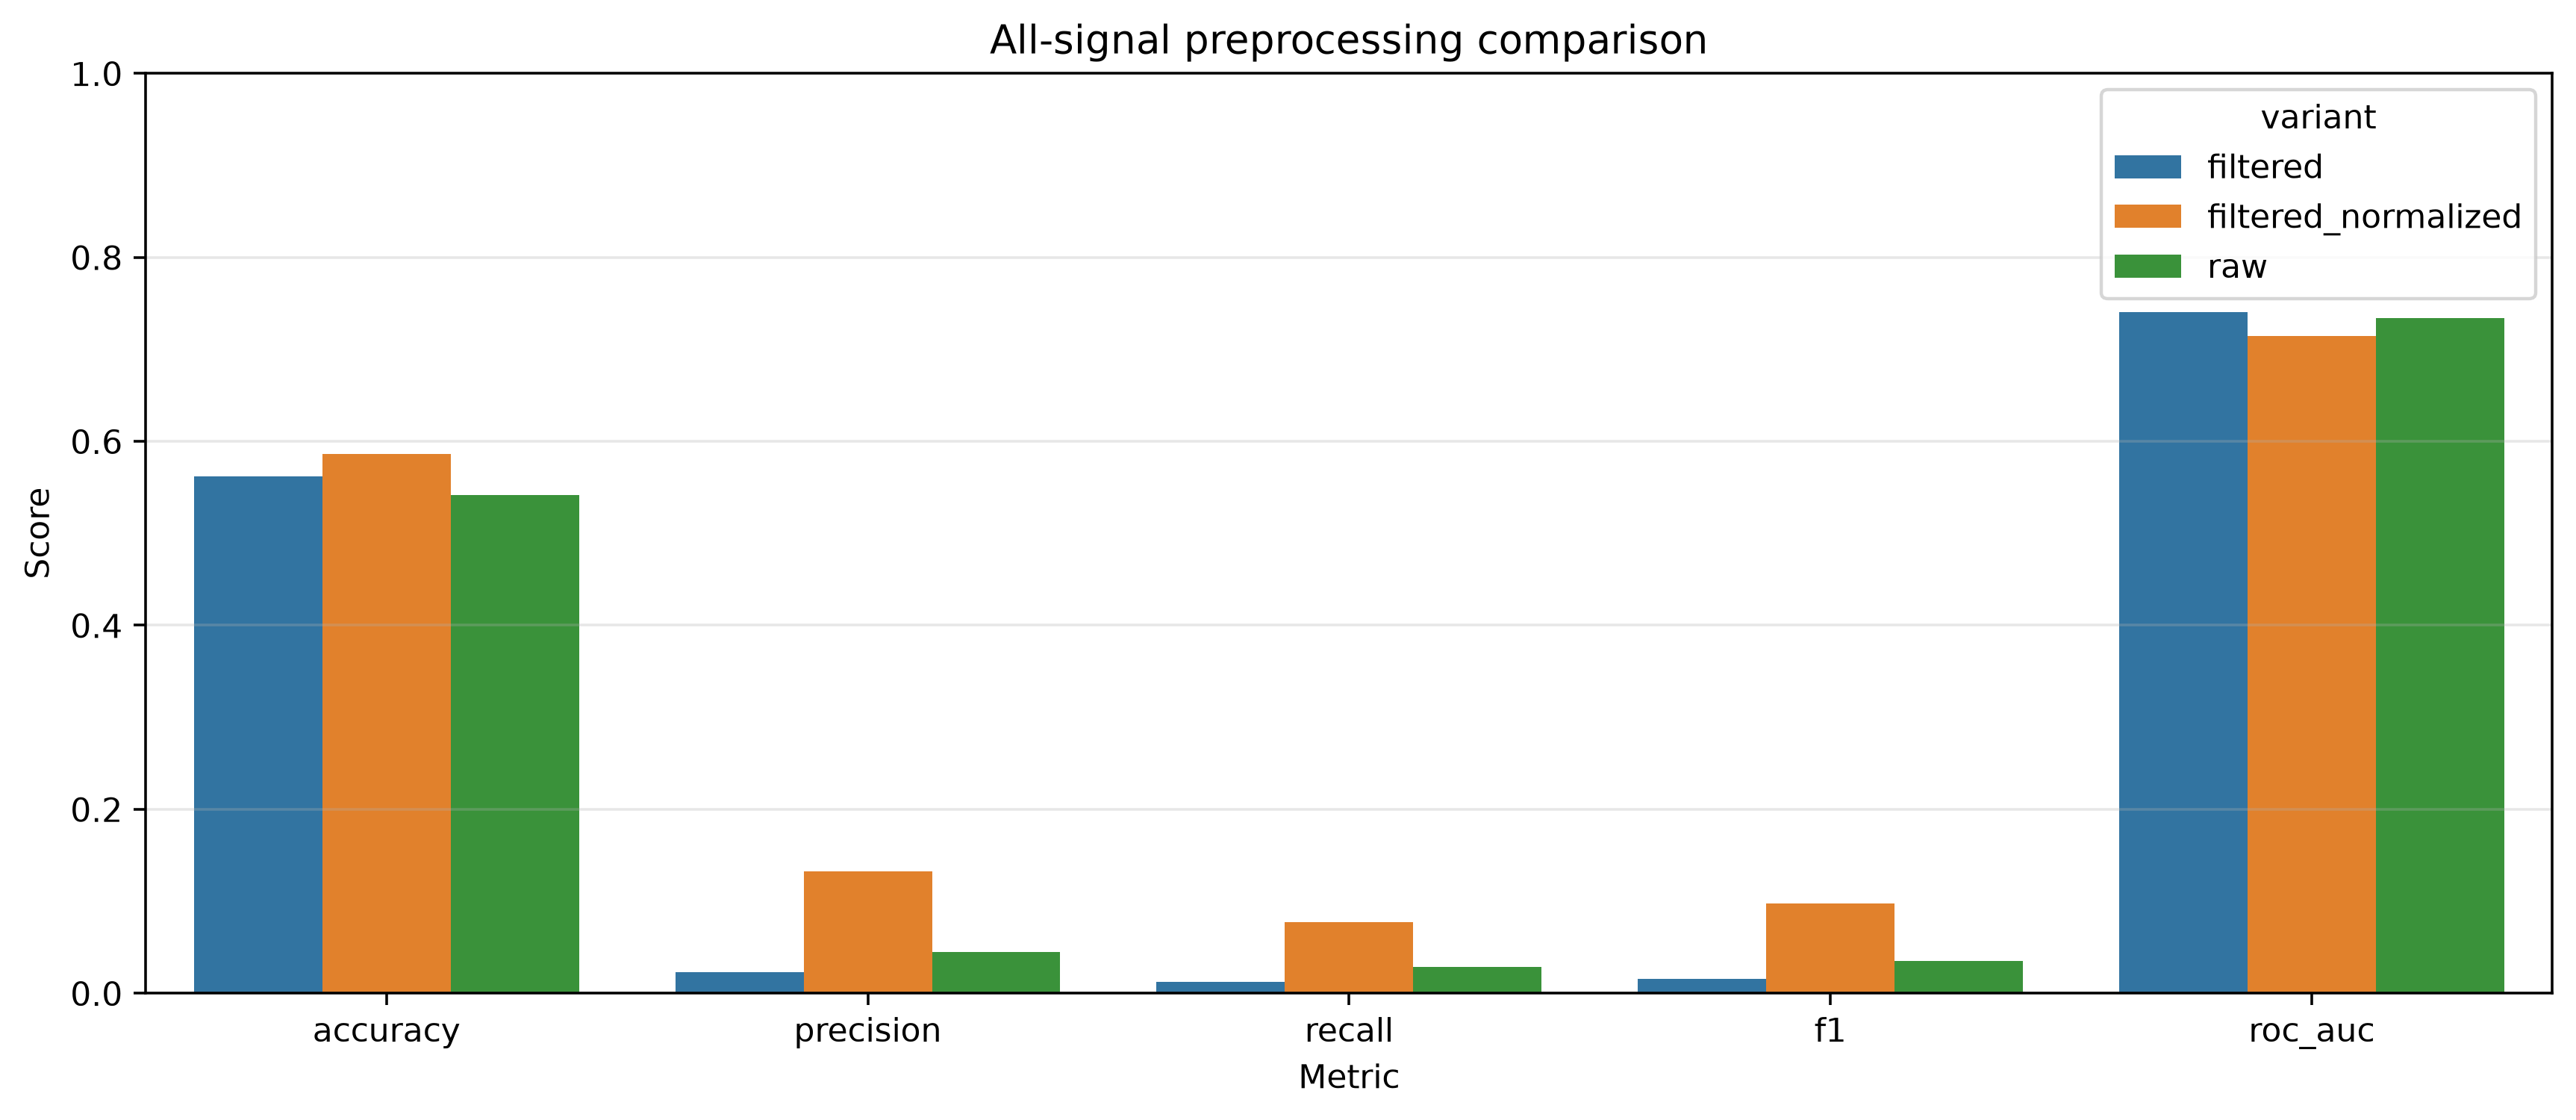
\includegraphics[width=\linewidth]{figures/overall_metric_comparison.png}
\caption{Overall held-out comparison of Raw, Filtered, and Filtered + Normalized all-signal inputs.}
\label{fig:overall-results}
\end{figure}

\begin{figure}[H]
\centering
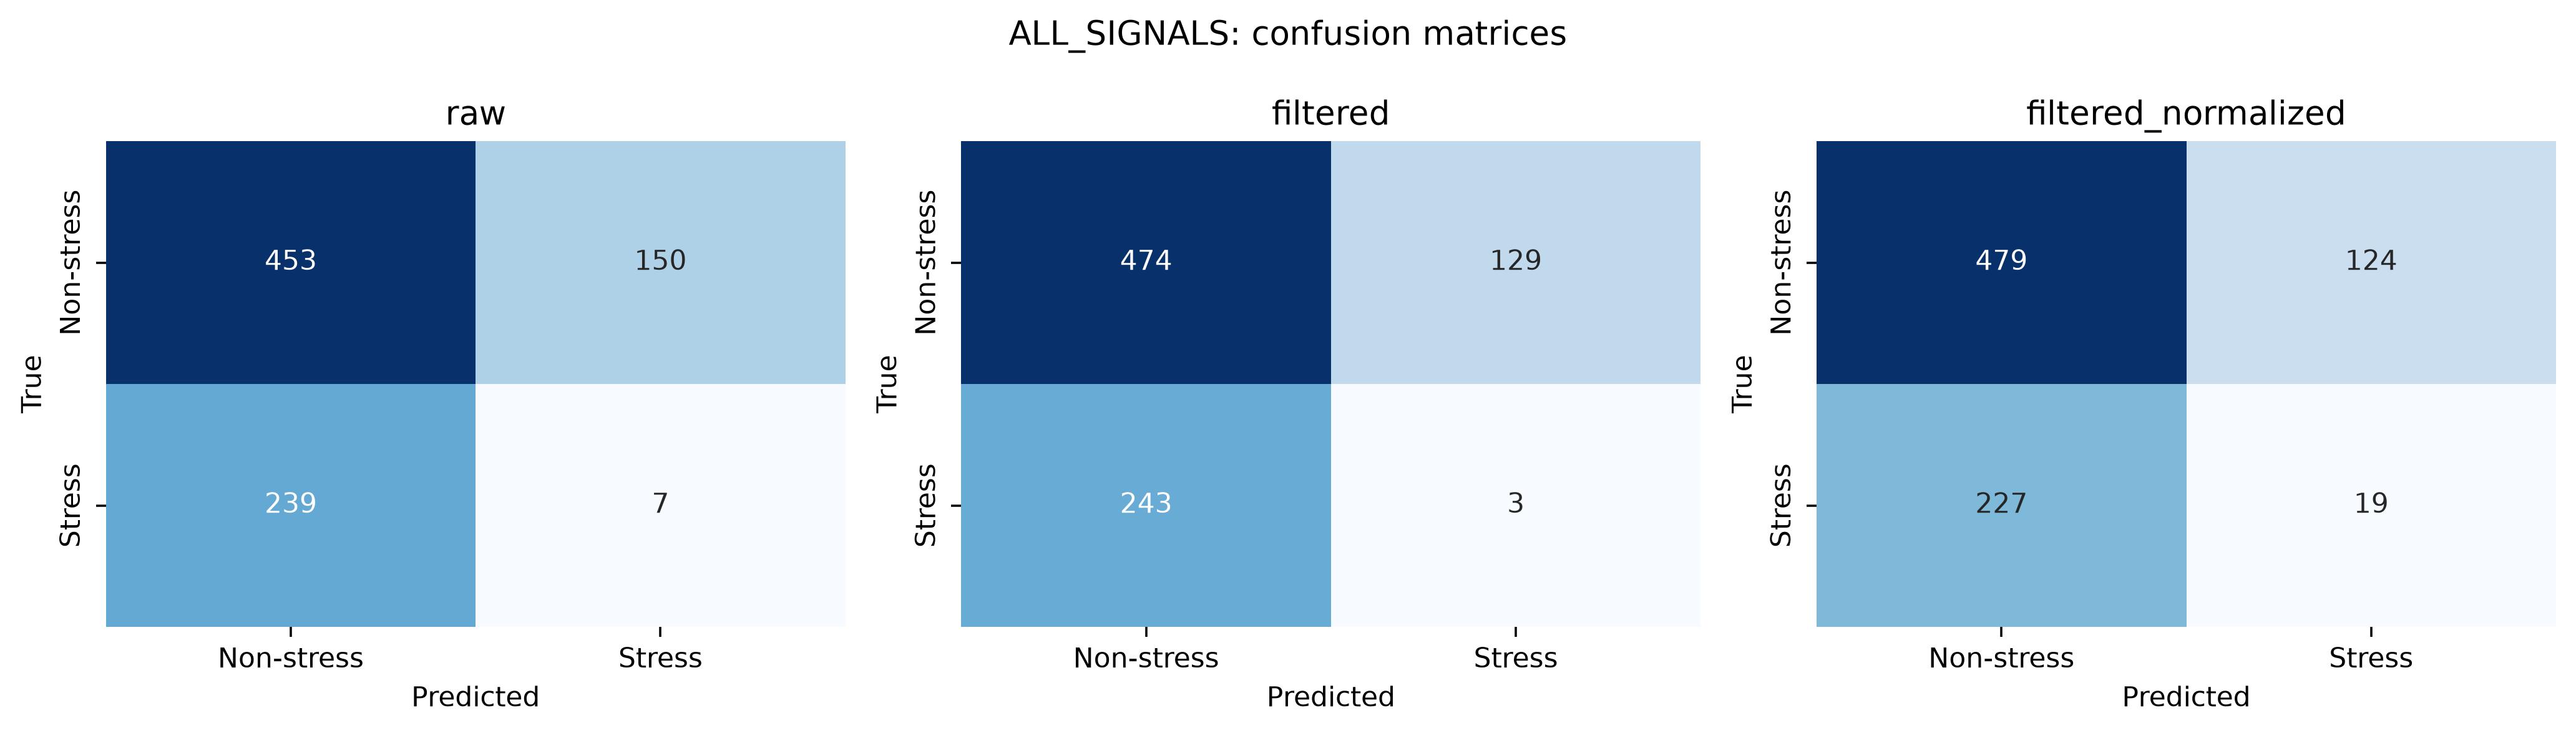
\includegraphics[width=0.95\linewidth]{figures/all_signals_confusion_matrices.png}
\caption{Confusion-matrix comparison for the all-signal experiments.}
\label{fig:confusion}
\end{figure}

\begin{figure}[H]
\centering
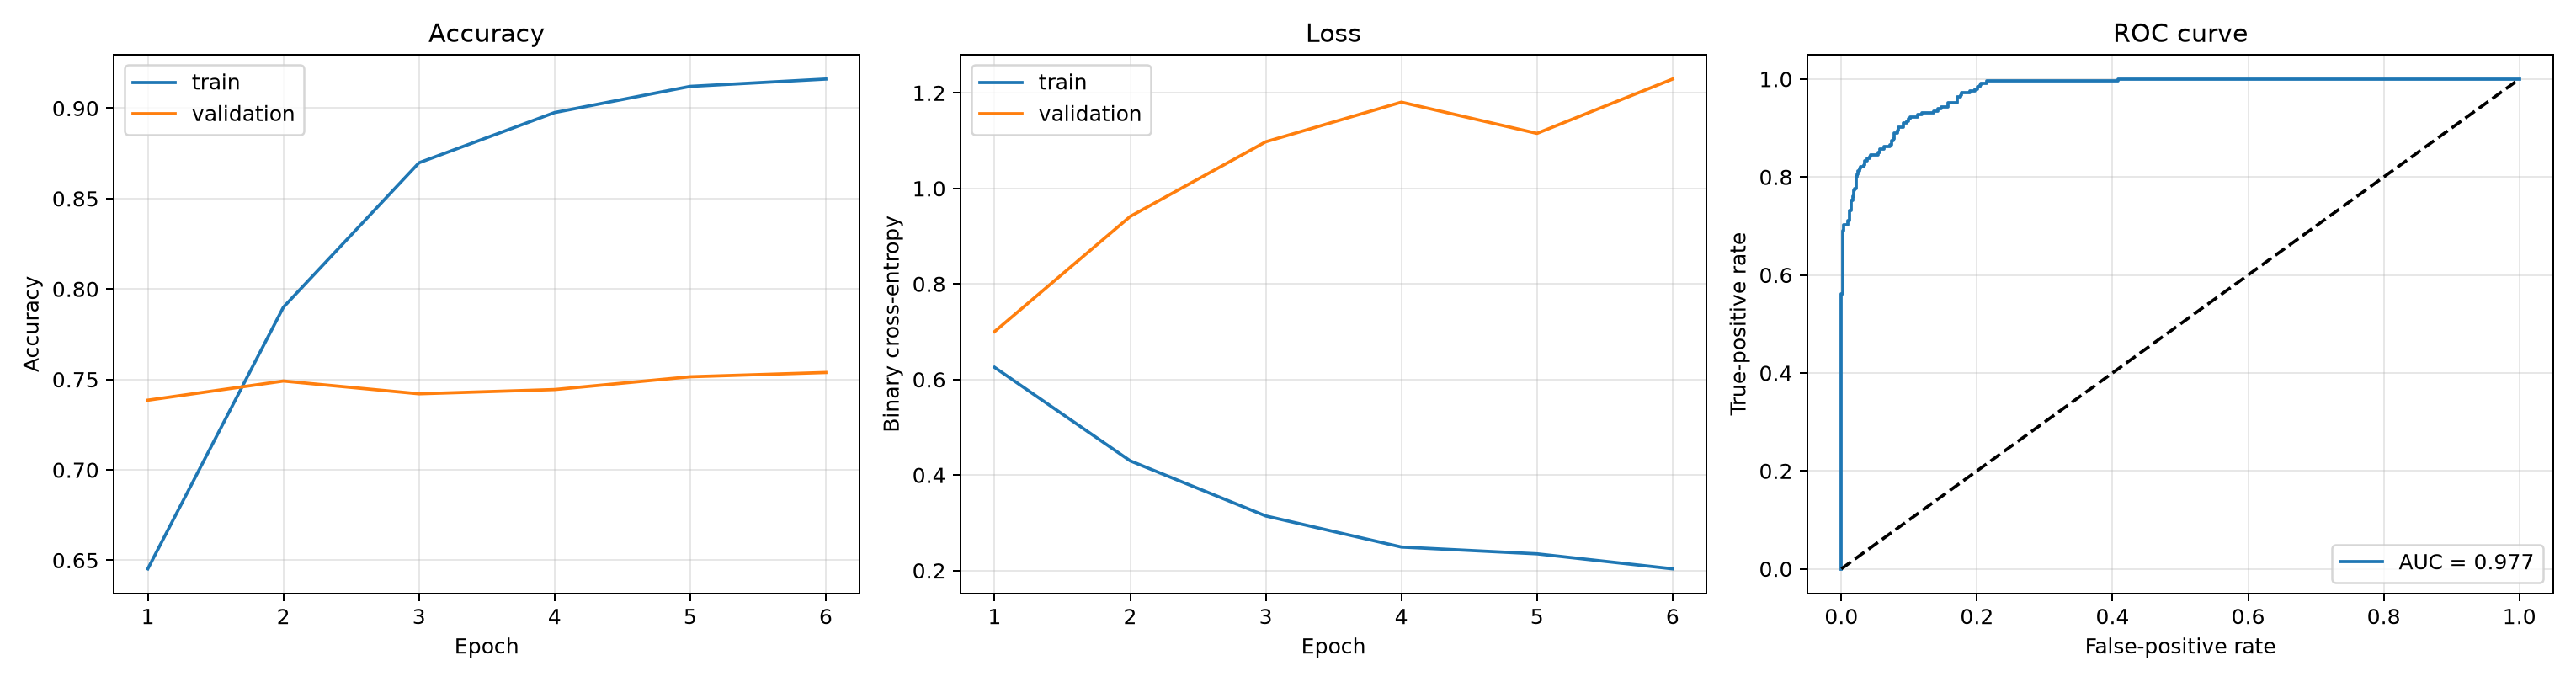
\includegraphics[width=0.95\linewidth]{figures/training_and_roc.png}
\caption{Existing model training history and ROC visualization retained from the repository output.}
\label{fig:roc}
\end{figure}

\section{Discussion}
The plots should be interpreted alongside the subject-independent performance table rather than in isolation. Filtering can improve robustness by reducing noise, while normalization makes feature scales comparable. The common 4-Hz ML branch supports a controlled comparison but cannot preserve high-frequency ECG or EMG morphology; future experiments should add dedicated native-rate features for those signals.

\section{Conclusion}
The repository now separates PNG visual evidence from the LaTeX narrative. The best preprocessing pipeline and strongest signal are selected from the recorded held-out F1 and ROC-AUC values, rather than from illustrative values. Future work should use more subjects, nested cross-validation, and physiological peak/HRV features where appropriate.

\begin{thebibliography}{9}
\bibitem{wesad} Schmidt, P. et al. Introducing WESAD, a multimodal dataset for wearable stress and affect detection. Proceedings of ICMI, 2018.
\end{thebibliography}
\end{document}
